
%(BEGIN_QUESTION)
% Copyright 2014, Tony R. Kuphaldt, released under the Creative Commons Attribution License (v 1.0)
% This means you may do almost anything with this work of mine, so long as you give me proper credit

Calculate the total amount of current that the battery must supply to this parallel circuit:

$$\includegraphics[width=15.5cm]{i01149x01.eps}$$

Now, using Ohm's Law, calculate total resistance ($R_{total}$) from total (source) voltage $V_{total}$ and total (source) current $I_{total}$.

\underbar{file i01149}
%(END_QUESTION)





%(BEGIN_ANSWER)

$I_{total} = 40.0 \hbox{ mA}$

\vskip 10pt

$R_{total} = 250 \> \Omega$

%(END_ANSWER)





%(BEGIN_NOTES)

While some students seem able to immediately grasp the concept of parallel resistances diminishing in (total) value, it is worthwhile to approach it from an Ohm's Law perspective as well to give other students a more formal rationale for this effect.

%INDEX% Electronics review: series and parallel circuits

%(END_NOTES)


